\newpage
\section{Problem D: Gene Folding}
\label{sec:Latex}
\subsection{Beschreibung der Problemdomäne}
\label{subsec:DokHeadGli}
Es wird eine einzelne genetische Sequenz vorgegeben, welche ausschließlich aus den Zeichen “A”, “C”, “G” und “T” besteht.

Die Darstellung der genetischen Sequenz kann bis zu vier Millionen Zeichen enthalten. Dabei kann die Sequenz in ihren Zeichen reduziert werden. Falls eine Stelle \textit{s} innerhalb der Sequenz existiert, für welche gilt, dass, ausgehend von \textit{s},  die linke Teilsequenz und die rechte Teilsequenz identisch sind und zusätzlich die linke Teilsequenz bis zum Präfix oder die rechte Teilsequenz bis zum Suffix reicht, darf die Sequenz bis zur Stelle \textit{s} reduziert werden. Dabei wird die Teilsequenz, welche bis zu einem Ende der Sequenz reicht, ausgeschnitten. Das Ziel besteht darin, eine minimale Sequenz zu bilden und die Länge dieser Sequenz auszugeben.
%
\subsection{Erkenntnisse}
\label{subsec:TextBefehle}
Bei der Eingabe handelt es sich um eine Sequenz von Zeichen und folglich um eine Zeichenkette. Die gegebene Zeichenkette kann durch Palindrome, welche beim Präfix starten oder beim Suffix enden, reduziert werden. Da es Palindrome sind, muss die linke und rechte Teilsequenz gleich lang sein. Zusätzlich ist die Stelle \textit{s}, welche auch als Faltindex bezeichnet werden kann, selbst kein Zeichen. Somit können nur Palindrome gerader Länge reduziert werden.

Nachdem die Zeichenkette bereits reduziert wurde, kann diese eventuell erneut reduziert werden. Angenommen, die erste Reduktion der Zeichenkette erfolgte ausgehend vom Präfix. \textit{Präfix’} bezeichnet den Präfix der bereits reduzierten Zeichenkette. Ausgehend vom \textit{Präfix’} muss ein weiteres Palindrom gerader Länge existieren, damit die bereits reduzierte Zeichenkette erneut reduziert werden kann. Jedes einzelne Palindrom, ausgehend vom Präfix zu reduzieren und danach erneut eine Reduktion zu überprüfen, wäre zu zeitintensiv. 

Angenommen, es existiert ein Palindrom, welches beim Präfix der ursprünglichen Zeichenkette startet. Dieses Palindrom wird als \textit{P1} bezeichnet. \textit{P1} hat die Länge \textit{L1}. Das Palindrom \textit{P1} reicht von der linke Grenze \textit{l1} bis zur rechten Grenze \textit{r1}. Der aktuelle Faltindex, bis zu welchem die Zeichenkette reduziert werden würde, wäre der Index \textit{i1}. Ausgehend davon, dass ein weiteres Palindrom existiert, gibt es zwei Möglichkeiten, sodass der Faltindex \textit{i1} erweitert werden kann.

Angenommen, ein weiteres Palindrom \textit{P2'} mit der Länge \textit{L2'} existiert. Für \textit{L2'} gilt: \textit{L2'} $\geq$ \textit{L1}+\textit{x}, mit $x \in \mathbb{N}$ und $x$ gerade. Für jedes folgende \textit{x} gelten die vorherigen Einschränkungen. Zusätzlich reicht \textit{P2'} von der linken Grenze \textit{l2'} bis zur rechten Grenze \textit{r2'}. Dabei gelten für \textit{l2'} und \textit{r2'}: \textit{l2'} = \textit{l1} und \textit{r2'} $\geq$ \textit{r1}+\textit{x}. Der Faltindex von \textit{P2'}, \textit{i2'}, entspricht dem Faltindex \textit{i1}+\textit{x}/2. Folglich ist \textit{i2'} > \textit{i1}. Wird ein Palindrom \textit{P2'} gefunden, welches das vorherige Palindrom \textit{P1} vollständig überdeckt, kann somit der Faltindex auf \textit{i2'} erweitert werden. 
 
Alternativ zu \textit{P2'} könnte ein Palindrom \textit{P2''} existieren. \textit{P2''} hat die Länge \textit{L2''} und die Grenzen \textit{l2''} und \textit{r2''}. Für die linke Grenze gilt: \textit{l1} <  \textit{l2''} $\leq$ \textit{i1}. Für den Index \textit{i2''} muss gelten: \textit{i2''} > \textit{i1}. \textit{P2''} würde somit nicht \textit{P1} vollständig überdecken, da \textit{P2''} nicht beim Präfix der ursprünglichen Zeichenkette startet. Allerdings könnte \textit{P1} theoretisch bis \textit{i1} reduziert werden. \textit{P2''} könnte ab dem neuen \textit{Präfix’} bis \textit{i2’'} reduziert werden, da \textit{l2’'} maximal dem \textit{Präfix’} entsprechen kann und zusätzlich \textit{i2’'} echt größer als \textit{i1} ist. Dementsprechend muss \textit{P2’'} ein Palindrom sein, welches am \textit{Präfix’} startet und einen größeren Index als \textit{i1} hat. Anstelle \textit{P1} zu reduzieren, kann \textit{i1} auf \textit{i2’'} erweiterte werden.

Zusammenfassend lässt sich festhalten, dass, falls die ursprüngliche Zeichenkette mehrfach vom Präfix reduziert werden kann, dies ohne die einzelnen Reduktionsschritte auszuführen erkannt ist. Voraussetzung dafür ist die Länge der einzelnen Palindrome der ursprünglichen Zeichenkette. Sind die Palindrome bekannt, kann in einem Durchlauf der Zeichenkette der maximale Faltindex ermittelt werden. Für die Palindrome, welche bis zum Suffix reichen, gilt dies analog.
%
\subsection{Lösungsansatz}
\label{subsec:Abb}
Zuerst muss die Sequenz eingelesen und als Zeichenkette gespeichert werden. Es sollen nun Palindrome verwendet werden, um diese Zeichenkette zu verkleinern. Mittels des Manacher-Algorithmus wird für jedes einzelne Zeichen einer Zeichenkette berechnet, wie lang die Palindrome sind, wenn die einzelnen Zeichen dem Faltindex des Palindromes entsprechen. Bekannt ist, dass ein Faltindex (Stelle \textit{s}) keinem Zeichen der Zeichenkette entsprechen kann. Daher wird die ursprüngliche Zeichenkette präpariert. Vor jedem Zeichen wird eine Raute gesetzt und am Ende wird die Zeichenkette mit einer Raute beendet. Der Manacher Algorithmus wird danach auf die präparierte Zeichenkette angewandt. Die Rauten zwischen den ursprünglichen Zeichen erfüllen somit die Aufgabe, die jeweilige Palindromlänge für die Palindrome gerader Länge zu speichern.
\begin{figure}[h]
    \centering
    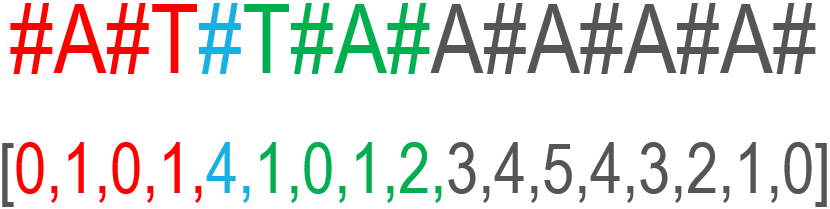
\includegraphics[width=8cm]{Bilder2/Abb1.PNG}
    \caption{Präparierte Zeichenkette mit zugehörigen Palindromlängen der einzelnen Zeichen}
    \label{fig:enter-label1}
\end{figure}
Die Abbildung~\ref{fig:enter-label1} zeigt beispielhaft die angepasste Version der ursprünglichen Sequenz (“ATTAAAAA”) und zusätzlich die berechneten Längen der Palindrome pro Zeichen. Die blaue vier beschreibt die Anzahl der identischen Zeichen auf beiden Seiten, ausgehend vom fünften Zeichen. Alle vier roten Zeichen stimmen, an dem fünften Zeichen gespiegelt, mit allen vier grünen Zeichen überein. Innerhalb der ursprünglichen Sequenz würde diese dem Palindrom “ATTA” entsprechen. Die blaue vier gibt somit, als Faltindex des Palindroms “ATTA”,  die Palindromlänge an. Der Manacher Algorithmus bestimmt die Palindromlängen auf Grundlage von Palindrom Eigenschaften.
\begin{figure}[h]
    \centering
    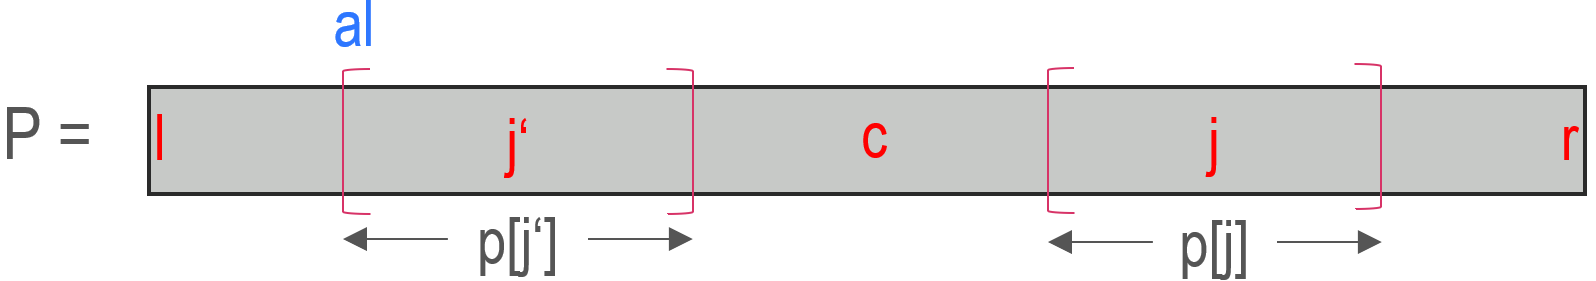
\includegraphics[width=11cm]{Bilder2/Abb2.PNG}
    \caption{Eigenschaften eines Palindromes}
    \label{fig:enter-label2}
\end{figure}

Angenommen, \textit{P} sei ein Palindrom. Die Grenzen werden durch \textit{l} und \textit{r} gekennzeichnet. Veranschaulicht durch Abbildung~\ref{fig:enter-label2} existiert ein Zeichen \textit{c}, welches das mittlere Zeichen des Palindromes \textit{P} darstellt. Bei Palindromen gerader Länge ist \textit{c} immer eine Raute. Für jedes Zeichen der rechten Teilzeichenkette des Palindromes, existiert ein identisches Zeichen innerhalb der linken Teilsequenz mit identischem Abstand zur \textit{c} und der jeweiligen Grenze. Diese zueinander korrespondierenden Zeichen müssen gleich sein, da beide innerhalb der Grenzen des Palindromes \textit{P} sich befinden. 

Der Manacher-Algorithmus bestimmt die Palindromlängen der Zeichen des Intervalls (\textit{c},\textit{r}) anhand der bekannten Palindromlängen der Zeichen des Intervalls (\textit{l},\textit{c}). In Abbildung~\ref{fig:enter-label2} wird beispielhaft die Palindromlänge des Zeichens \textit{j} gesucht. Für das identische Zeichen \textit{j'}, der linken Teilzeichenkette, ist die Palindromlänge, \textit{p[j’]}, bekannt. Die linke Grenze des inneren Palindromes von \textit{j} wird \textit{al} bezeichnet. Solange \textit{al} echt größer als \textit{l} ist, muss die rechte Grenze des inneren Palindromes von \textit{j} echt kleiner sein als \textit{r}. Sollte \textit{al}>\textit{l} gelten, muss die Palindromlängen \textit{p[j]} der Palindromlänge \textit{p[j’]} entsprechen.

Entspricht \textit{al} der linken Grenze \textit{l} oder überschreitet \textit{al} diese Grenze, muss die rechte Grenze \textit{r} erweitert werden. In diesem Fall kann \textit{p[j]} gleich oder größer als \textit{p[j’]} sein. Weitere Zeichen, nach der aktuellen rechten Grenze, könnten noch zum Palindrom \textit{p[j’]} gehören und daher kann \textit{p[j’]} größer ausfallen als \textit{p[j]}. 

Der Manacher-Algortihmus verwendet die Feld-Datenstruktur, um alle Palindromlängen zu speichern. Das Feld ist die Ausgabe des Manacher-Algorithmus. Für die minimale Sequenz, werden die maximalen Faltindizes ausgehend vom Präfix und Suffix benötigt. Die maximalen Faltindizes werden mit Präfix-Faltindex beziehungsweise Suffix-Faltindex abgekürzt. Der Präfix-Faltindex wird innerhalb eines Durchlaufs des Feldes ermittelt, aufgrund der Erkenntnisse, wie ein Präfix-Faltindex erweitert werden kann. Die präparierte Zeichenkette wird bis zum maximalen Präfix-Faltindex reduziert. Bezeichnet wird die resultierende Zeichenkette als RZ. Für RZ wird der maximale Suffix-Faltindex berechnet. Wird die resultierende Zeichenkette umgekehrt, berechnet sich der maximale Suffix-Faltindex identisch zum Präfix-Faltindex. Der  Suffix-Faltindex passt nicht zur präparierten Zeichenkette, da diese nicht umgekehrt wurde. Der Suffix-Faltindex der präparierten Zeichenkette ermittelt sich durch:
\begin{align}
(\text{Präfix-Faltindex}+\text{Größe RZ} - \text{Suffix-Faltindex der umgekehrten Zeichenkette} - 1)
\end{align}
Das Ergebnis berechnet sich aus den Faltindizes der präparierten Zeichenkette und wird durch zwei geteilt, da die präparierte Zeichenkette die Rauten enthält, welche die ursprünglichen Sequenz nicht enthielt.
\begin{align}
((\text{Suffix-Faltindex}) - (\text{Präfix-Faltindex})) / 2
\end{align}
%
\subsection{Implementierung}
\label{subsec:TextBefehle}
Die verwendeten Methoden werden im Folgenden vereinfacht dargestellt. Eine vollständige Implementierung in C++ ist im Anhang zu finden.
\begin{lstlisting}
//präpariert eine Zeichenkette
//example: input=abba; output=#a#b#b#a#
string preString(input){
    output = "#";
    //durchlaufe jedes Zeichen der ursprünglichen Zeichenkette    
    for(char c : input){
        output += c;
        output += '#';
    }    
    return output;
}
//berechnet Palindromlänge für jedes Zeichen einer Zeichenkette
vector<int> manacherAlgorithm(str){
    lengths = Ergebnisfeld
    c = Zentrum des längsten Palindromes
    r = rechte Grenze des längsten Palindromes
    //iteriert über jedes Zeichen der Eingabe
    for(int i=0; i<str.length(); i++){ 
        mirror = Position des identischen Zeichen der linken Teilzeichenkette
        //überprüft, ob sich das aktuelles Zeichen innerhalb des längsten 
        //Palindromes befindet
        if(i<r){
            lengths[i] = min(r-i, lengths[mirror]);
        }
        right = rechte Grenze des längsten Palindromes
        left = linke Grenze des längsten Palindromes
        //Palindromerweiterung des einzelnen Zeichens
        while(left>=0 && right<str.length() && str[right] == str[left]){
            lengths[i]++;
            right++;
            left--;
        }
        //falls Palindromerweiterung über right hinausgeht => Grenzen anpassen
        if(i+lengths[i]>r){
            c = i;
            r = i+lengths[i];
        }
    }
    return lengths;
}
//ermittelt den maximalen Präfix-Faltindex
int maxCut(vector<int>& lengths, string& str){
    max = 0 //Startwert
    //durchläuft alle Palindromlängen der Palindrome gerader Länge
    for(int i=2; i<=(lengths2.size()); i+=2){ 
        //überprüft, ob der Faltindex erweitert werden kann
        if((lengths2[i]>0 && lengths2[i] == i) || lengths2[i]+max >= i){
            max = i;
        }
    }
    return max;
}
\end{lstlisting}
%
\subsection{Laufzeit}
\label{subsec:TextBefehle}
Das Präparieren einer Zeichenkette benötigt einen Durchlauf aller Zeichen der ursprünglichen Zeichenkette. Der Manacher Algorithmus benötigt einen Durchlauf aller Zeichen der präparierten Zeichenkette und aktualisiert die Palindromlängen der Zeichen innerhalb konstanter Zeit. Palindromlängen einzelner Zeichen, werden direkt übernommen, falls die Grenzen des Palindromes innerhalb der bekannten Grenzen \textit{l} und \textit{r} liegen. Geht die rechte Grenze des inneren Palindromes über die rechte Grenze \textit{r} hinaus, so wird diese erweitert. Dementsprechend hat der Manacher Algorithmus eine Laufzeit von $\mathcal{O}(2N+1)$ [1], wenn \textit{N} die Eingabelänge der ursprünglichen Zeichenkette ist. Ein maximaler Präfix-Faltindex wird ebenfalls innerhalb eines Durchlauf jeder zweiten Zahl des Feldes, welches vom Manacher Algorithmus berechnet wurde, ermittelt. Jede Zahl entspricht einem Zeichen, daher benötigt die Berechnung eines maximalen Präfix-Faltindex nur einen Durchlauf der ursprünglichen Zeichenkette. Unter der Annahme, dass die ursprüngliche Sequenz aus \textit{N} Zeichen besteht, lässt sich eine asymptotische Laufzeit von $\mathcal{O}(N)$ ermitteln.
%
\subsection{Testergebnisse}
\label{subsec:TextBefehle}
Die Implementierung konnte ausschließlich anhand der gegebenen Testfälle geprüft werden. Mit Hilfe eines Python-Skripts wurden alle beispielhaften Eingaben ausgeführt. Der Anhang enthält eine Tabelle mit der Laufzeit pro Eingabe in Sekunden, zusammen mit den Resultaten. Jedes Resultat wurde mit dem erwarteten Wert verglichen. Die Resultate stimmten immer mit den erwarteten Werte überein. Außerdem benötigt keine der Eingaben für die Ausführung mehr als die vorgegebenen fünf Sekunden.
%